%%%%%%%%%%%%%%%%%%%%%%%%%%%%%%%%%%%%%%%%%
% University Assignment Title Page 
% LaTeX Template
% Version 1.0 (27/12/12)
%
% This template has been downloaded from:
% http://www.LaTeXTemplates.com
%
% Original author:
% WikiBooks (http://en.wikibooks.org/wiki/LaTeX/Title_Creation)
%
% License:
% CC BY-NC-SA 3.0 (http://creativecommons.org/licenses/by-nc-sa/3.0/)
% 
% Instructions for using this template:
% This title page is capable of being compiled as is. This is not useful for 
% including it in another document. To do this, you have two options: 
%
% 1) Copy/paste everything between \begin{document} and \end{document} 
% starting at \begin{titlepage} and paste this into another LaTeX file where you 
% want your title page.
% OR
% 2) Remove everything outside the \begin{titlepage} and \end{titlepage} and 
% move this file to the same directory as the LaTeX file you wish to add it to. 
% Then add \input{./title_page_1.tex} to your LaTeX file where you want your
% title page.
%
% template taken from https://www.overleaf.com/latex/examples/title-page-with-logo/hrskypjpkrpd#.WDXHQKIrLdc
%%%%%%%%%%%%%%%%%%%%%%%%%%%%%%%%%%%%%%%%%
%\title{Title page with logo}
%----------------------------------------------------------------------------------------
%   PACKAGES AND OTHER DOCUMENT CONFIGURATIONS
%----------------------------------------------------------------------------------------

\documentclass[12pt]{article}
\usepackage[english]{babel}
\usepackage[utf8x]{inputenc}
\usepackage{algpseudocode}
\usepackage{algorithm}
\usepackage{algorithmicx}
\usepackage{amsmath}
\usepackage{courier}
\usepackage{graphicx}
\usepackage{hyperref}
\usepackage{listings}
\usepackage{url}
\usepackage[colorinlistoftodos]{todonotes}

\begin{document}

\begin{titlepage}

\newcommand{\HRule}{\rule{\linewidth}{0.5mm}} % Defines a new command for the horizontal lines, change thickness here

\center % Center everything on the page
 
%----------------------------------------------------------------------------------------
%   HEADING SECTIONS
%----------------------------------------------------------------------------------------

\textsc{\LARGE The University of Texas at Austin}\\[1.5cm] % Name of your university/college
\textsc{\Large Distributed Systems}\\[0.5cm] % Major heading such as course name
\textsc{\large Software Engineering - Option III}\\[0.5cm] % Minor heading such as course title

%----------------------------------------------------------------------------------------
%   TITLE SECTION
%----------------------------------------------------------------------------------------

\HRule \\[0.4cm]
{ \huge \bfseries Raft - An Understandable Distributed Consensus Protocol}\\[0.4cm] % Title of your document
\HRule \\[1.5cm]
 
%----------------------------------------------------------------------------------------
%   AUTHOR SECTION
%----------------------------------------------------------------------------------------

\begin{minipage}{0.4\textwidth}
\begin{flushleft} \large
\emph{Authors:}\\
Howie \textsc{Benefiel}\\
Patrick \textsc{Sigourney} % Your name
\end{flushleft}
\end{minipage}
~
\begin{minipage}{0.4\textwidth}
\begin{flushright} \large
\emph{Professor:} \\
Dr. Vijay \textsc{Garg} % Supervisor's Name
\end{flushright}
\end{minipage}\\[2cm]

% If you don't want a supervisor, uncomment the two lines below and remove the section above
%\Large \emph{Author:}\\
%John \textsc{Smith}\\[3cm] % Your name

%----------------------------------------------------------------------------------------
%   DATE SECTION
%----------------------------------------------------------------------------------------

{\large \today}\\[2cm] % Date, change the \today to a set date if you want to be precise

%----------------------------------------------------------------------------------------
%   LOGO SECTION
%----------------------------------------------------------------------------------------


\includegraphics{logo.png}\\[1cm] % Include a department/university logo - this will require the graphicx package
 
%----------------------------------------------------------------------------------------

\vfill % Fill the rest of the page with whitespace

\end{titlepage}


\begin{abstract}
    Paxos has been the industry-standard protocol for implementing distributed consensus for the past 25 years.
    Though the basics of single-decree consensus are easily enough grokked, delving into why it works, forming a replicated log or implementing membership changes is fraught with unproven ambiguity.
    Raft was designed with a singular design goal, understandability.
    To achieve this goal of optimizing for understandability, the authors employed two techniques, problem decomposition and minimization of state space.
    For this paper, we examined and implemented their protocol.
    We found their protocol performed as well as they claimed and it was much easier to fundamentally grok than Paxos.
\end{abstract}

\section{Introduction}

The primary focus of distributed consensus is to take an unreliable machine and replicate it so that it becomes a cluster of individually unreliable but collectively reliable machines.
The most studied model for this is the replicated state machine model.
In this model, each machine has some internal state which can be changed by external stimulus.
Perhaps obviously, the state of these state machines should be replicated by all the machines in the cluster.
At a high level, the duty of a distributed consensus protocol is to ensure the state stays consistent across all the machines in the cluster.

The core data structure in a practical consensus algorithm, and indeed Raft, is the replicated log.
The replicated log contains all the commands that have been run against the cluster.
If a machine were to start at the beginning of the log and execute each command, in order, in its log, that machine should arrive at a state consistent with other machines in the cluster.
At a more practical level, a distributed consensus protocol will keep these replicated logs consistent across the cluster.

FLP states that an asynchronous distributed system can not tolerate failure and satisfy agreement, validity and termination. \cite{flp-theorem}
So, consensus algorithms generally satisfy:
\begin{enumerate}
    \item \textit{Safety} They always return a correct result.
    If a client randomly queries any server for the state of the system, the result should be the same regardless of which machine was queried.
    \item \textit{Availability} If a majority of the servers are available, the system, as a whole should be available.
    \item \textit{Time Invariance} The system should not depend on the physical timing of events.
    \item \textit{Quorum Rate-Limiting} The response to the client should be returned once quorum is reached, not when all machines have responded.
\end{enumerate}


First, they on decomposed the primary problem, distributed consensus, into a couple independent sub-problems.
Second, they minimized the state space of the algorithm.

\section{Previous Work}


\section{Algorithm}


\subsection{Everything below this is just an example}


% todo remove - this is just an example of an image
\begin{figure}
\centering{}
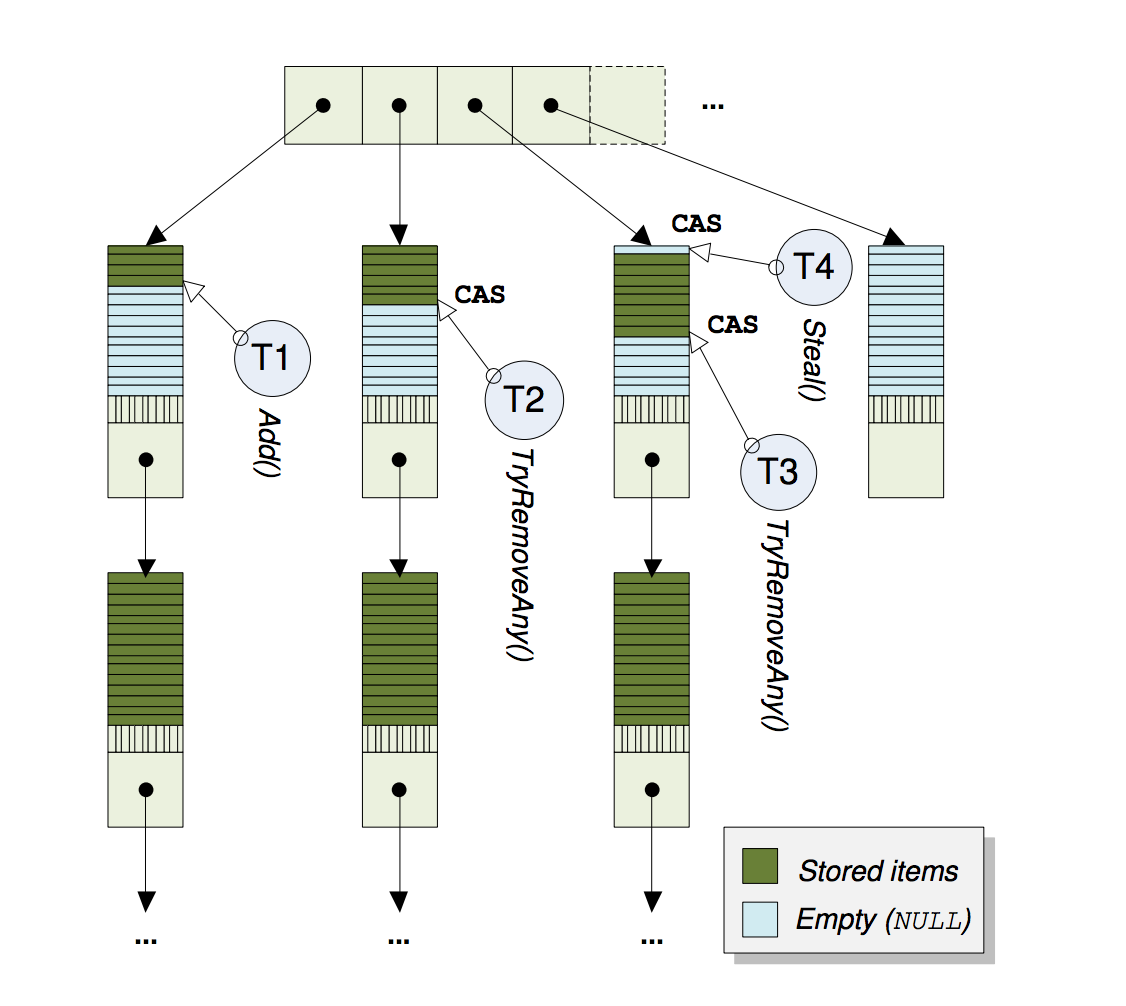
\includegraphics[width=0.75\textwidth]{datastructure.png}
\caption{\label{fig:datastruct}Above is the graphical representation of the basic data structure. The top array is globalHeadBlock. The linked list nodes below the array are the blocks. The green and blue cells are the objects being operated on.}
\end{figure}

% todo remove - this is just an example of having inline "code" and references etc
\subsection{Basic Operations on the Data Structure}

There are two basic operations which can be used on a bag, \texttt{Add(item)} and \texttt{TryRemoveAny()}.
\texttt{Add(item)} will add an item anywhere in the data structure, as expected.
The \texttt{Add(item)} algorithm with detailed comments is shown in Algorithm~\ref{alg:add}.
When adding or removing from the data structure, the threads keep track of the position in the block they can access
and the first block in their linked list through the thread-local variables, \texttt{threadHead}
and \texttt{threadBlock}, respectively. This is shown in Fig.~\ref{fig:datastruct} as the thread-numbered
circles pointing to a position. One thing to note about \texttt{Add()} is that items will always
only be added to the first block in the linked list and at most 1 thread will be adding to a block.

\texttt{TryRemoveAny()} is used to remove any random item from the data structure and return it.
This is shown with detailed comments in Algorithm~\ref{alg:remove}.
Now the situation may arise where a thread's linked list only contains empty blocks.
For this situation, the \texttt{TryRemoveAny} operation provides functionality via the
\texttt{Steal()} method to steal from another thread's block. This is shown
in Algorithm~\ref{alg:remove} at line~\ref{remove:line:steal}.

% todo remove - this is jsut an example of embedding an algoritm
\begin{algorithm}
\caption{\texttt{Add(item)} Operation}
\label{alg:add}
\begin{algorithmic}[1]
\If {$threadHead == BLOCK\_SIZE$} \Comment{the current block is full}
    \State Create new block and add it at the head of the linked list
    \State $threadHead \gets 0$
\EndIf
\State $threadBlock[threadHead] \gets item$ \Comment{Insert value at current threadHead}
\State $threadHead \gets threadHead + 1$ \Comment{Advance threadHead to next position}
\end{algorithmic}
\end{algorithm}

\begin{algorithm}
\caption{\texttt{TryRemoveAny()} Operation}
\label{alg:remove}
\begin{algorithmic}[1]
\Loop
    \If {$ threadHead < 0$}
        \If {$ head < 0$ and next block $==$ null} \Comment{End of linked list}
            \State \Return Steal() \Comment{Go to steal} \label{remove:line:steal}
        \EndIf
        \State $threadBlock \gets threadBlock.next$ \Comment{advance position in list}
        \State $threadHead \gets BLOCK\_SIZE$ \Comment{last position in block}
    \EndIf
    \State $item \gets threadBlock[threadHead]$ \Comment{Retrieve item from block}
    \If { item $\ne$ null and CAS(threadBlock[threadHead],item,null) }
        \State \Return item \Comment{If CAS successful, return the item}
    \Else
        \State $threadHead \gets threadHead - 1$ \Comment{If not, try next and loop}
    \EndIf
\EndLoop
\end{algorithmic}
\end{algorithm}


\section{Implementation}



\section{Conclusion}



\appendix

%\section{Thread-Local Example}
%\label{sec:tls}
%\lstinputlisting[language=Java, firstline=366, lastline=382]{../../java-bag/src/SwedishBag.java}
% \section{Some \LaTeX{} Examples}
% \label{sec:examples}

% \subsection{Sections}

% Use section and subse{}ction commands to organize your document. \LaTeX{} handles all the formatting and numbering automatically. Use ref and label commands for cross-references.

% \subsection{Comments}

% Comments can be added to the margins of the document using the \todo{Here's a comment in the margin!} todo command, as shown in the example on the right. You can also add inline comments too:

% \todo[inline, color=green!40]{This is an inline comment.}

% \subsection{Tables and Figures}

% Use the table and tabular commands for basic tables --- see Table~\ref{tab:widgets}, for example. You can upload a figure (JPEG, PNG or PDF) using the files menu. To include it in your document, use the includegraphics command as in the code for Figure~\ref{fig:frog} below.

% % Commands to include a figure:
% \begin{figure}
% \centering
% \includegraphics[width=0.5\textwidth]{frog.jpg}
% \caption{\label{fig:frog}This is a figure caption.}
% \end{figure}

% \begin{table}
% \centering
% \begin{tabular}{l|r}
% Item & Quantity \\\hline
% Widgets & 42 \\
% Gadgets & 13
% \end{tabular}
% \caption{\label{tab:widgets}An example table.}
% \end{table}

% \subsection{Mathematics}

% \LaTeX{} is great at typesetting mathematics. Let $X_1, X_2, \ldots, X_n$ be a sequence of independent and identically distributed random variables with $\text{E}[X_i] = \mu$ and $\text{Var}[X_i] = \sigma^2 < \infty$, and let
% $$S_n = \frac{X_1 + X_2 + \cdots + X_n}{n}
%       = \frac{1}{n}\sum_{i}^{n} X_i$$
% denote their mean. Then as $n$ approaches infinity, the random variables $\sqrt{n}(S_n - \mu)$ converge in distribution to a normal $\mathcal{N}(0, \sigma^2)$.

% \subsection{Lists}

% You can make lists with automatic numbering \dots

% \begin{enumerate}
% \item Like this,
% \item and like this.
% \end{enumerate}
% \dots or bullet points \dots
% \begin{itemize}
% \item Like this,
% \item and like this.
% \end{itemize}

% We hope you find write\LaTeX\ useful, and please let us know if you have any feedback using the help menu above.

\bibliographystyle{plain}
\bibliography{references}

\end{document}
